\documentclass[12pt]{article} % use larger type; default would be 10pt

%packages
\usepackage[utf8]{inputenc} % set input encoding (not needed with XeLaTeX)
\usepackage{fancyhdr}
\usepackage{float}
\usepackage{geometry}
\usepackage{ulem}
\usepackage{soul}
\usepackage{color}
\usepackage{graphicx}
\usepackage{hyperref}
\usepackage{array}
\usepackage{caption}
\usepackage{titling}
\usepackage{enumerate} 
\usepackage[dvipsnames]{xcolor}
\usepackage{amsmath}
\usepackage{amssymb}
\usepackage[compact]{titlesec}


 %put box around figure captions
\makeatletter
\long\def\@makecaption#1#2{%
  \vskip\abovecaptionskip
  \sbox\@tempboxa{\fbox{#1: #2}}%
  \ifdim \wd\@tempboxa >\hsize
    \fbox{\parbox{\dimexpr\linewidth-2\fboxsep-2\fboxrule}{#1: #2}}\par
  \else
    \global \@minipagefalse
    \hb@xt@\hsize{\hfil\box\@tempboxa\hfil}%
  \fi
  \vskip\belowcaptionskip}
\makeatother

%reduce space between 
\titlespacing{\section}{0pt}{*1}{*0}
\titlespacing{\subsection}{0pt}{*1}{*0}
\titlespacing{\subsubsection}{0pt}{*0}{*0}


%no indent and modify distance between paragraphs
\setlength\parindent{0pt}
\setlength\parskip{12pt}

%set margins and line spacing
\geometry{margin=1in}
\linespread{1.2}
\geometry{letterpaper}

%math operators
\DeclareMathOperator{\E}{\mathbb{E}}

%set up header and page numbering
\pagestyle{fancy}
\lhead{CS 155 Set 1}
\rhead{Timothy Liu}
\pagenumbering{arabic}



\title{CS155 Set 3}
\author{Timothy Liu}

\begin{document}


\maketitle

\newpage

\section{Problem 1}
\subsection{Problem A}

\begin{figure}[H]
	\makebox[\textwidth][c]{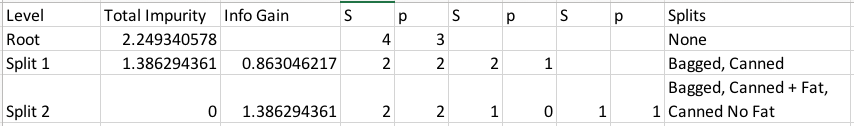
\includegraphics[width=7in]{1ai.png}}
	\vspace{-10mm}
	\caption{Impurity at each step of decision tree using log entropy.}
\end{figure}

\begin{figure}[H]
	\makebox[\textwidth][c]{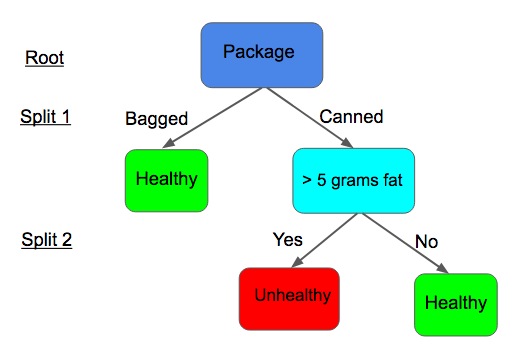
\includegraphics[width=4.2in]{1aii.png}}
	\vspace{-10mm}
	\caption{Illustration of decision tree.}
\end{figure}
\subsection{Problem B}
No, a decision tree is not always preferred for classification. There are some datasets which are easier to classify linearly but difficult to do with a decision tree.

\begin{figure}[H]
	\makebox[\textwidth][c]{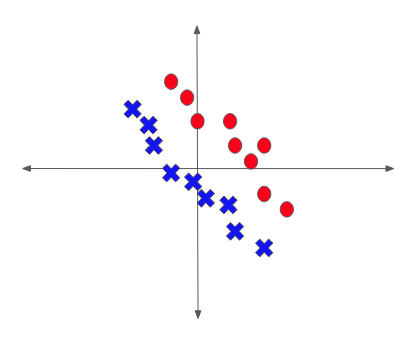
\includegraphics[width=4.2in]{1b.png}}
	\vspace{-10mm}
	\caption{Dataset easy to separate with linear classifier and more complex for a decision tree.}
\end{figure}

\subsection{Problem C}
\subsubsection{i}
\begin{figure}[H]
	\makebox[\textwidth][c]{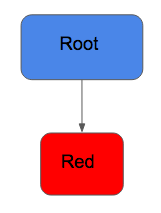
\includegraphics[width=2in]{1ci.png}}
	\vspace{-10mm}
	\caption{Decision tree trained using Gini index.}
\end{figure}

There are no splits that reduce the Gini index. At the root, half of the points are misclassified. All of the possible first splits will have two branches that have half of the points misclassified, so there is no reduction in the Gini Index. The decision tree may choose to label all of the points red or all of the points green. The classification error is $\frac{1}{2}$.

Yes. The problem with the Gini index is that it cannot break ties; the decision tree stalls because the first split results in two nodes that sum together with the same impurity as the root node. An impurity function where impurity scales with and falls with the number of points could generate the above decision tree. Such a function would not end with a tie, since the splits would have a smaller impurity because each node has a smaller number of points. The pro of such an approach is that it focuses more on the number of misclassified points rather than the fraction, so it places less weight on further splitting nodes that may have high impurity but sparse points. The con is that such an approach would have results dependent on the size of the training set.

\subsubsection{ii}

\begin{figure}[H]
	\makebox[\textwidth][c]{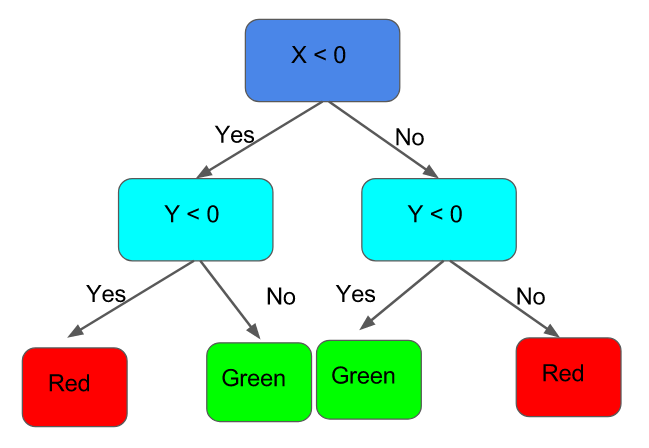
\includegraphics[width=4.2in]{1cii.png}}
	\vspace{-10mm}
	\caption{2 level decision tree that perfectly categorizes the data.}
\end{figure}

\subsubsection{iii}
The most difficult 2D data set to train is a 10 by 10 checkerboard array where each point is classified differently from the points directly left, right, above, and below it. 98 internal nodes are needed to perfectly classify such a set. Since each split in the final tree will only contain a single point, a node is needed to split off every point. One node is the root node, and an additional 98 internal nodes are needed to split the remaining points.

\subsection{Problem D}
The worst case scenario for training time is $O(N \times D)$. There are up to N-1 ways to split a dataset with N points, since a decision boundary can be between any two adjacent points. This process must be repeated across all D dimensions, so the worse case is the product $(N - 1) \times D$ which asymptotically approaches $O(N \times D)$.

\section{Problem 2}

\subsection{Problem A}
\begin{figure}[H]
	\makebox[\textwidth][c]{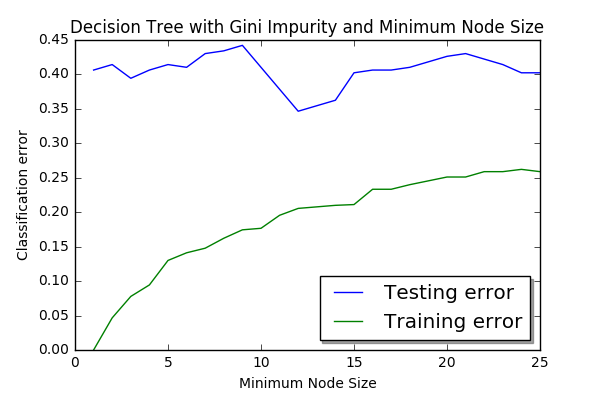
\includegraphics[width=5in]{2a.png}}
	\vspace{-10mm}
	\caption{Decision tree with varying minimum leaf node size.}
\end{figure}
As the minimum node size increases, the training error generally increases. However, the testing error hits a minimum at a minimum node size of 13.

\subsection{Problem B}

\begin{figure}[H]
	\makebox[\textwidth][c]{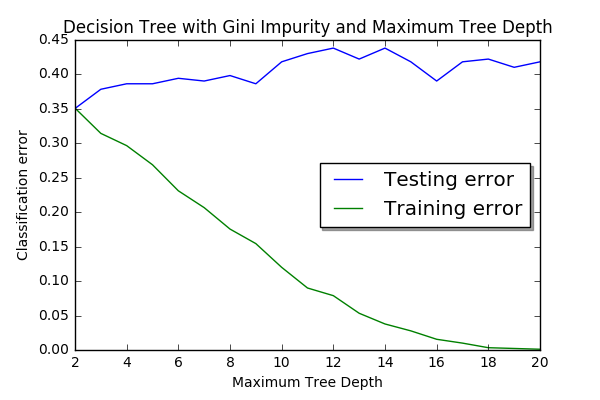
\includegraphics[width=4.2in]{2b.png}}
	\vspace{-10mm}
	\caption{Decision tree with varying maximum tree depth.}
\end{figure}

As maximum tree depth increases, the training error falls to zero. However, the testing error is lowest when the maximum tree depth is only 2.

\subsection{Problem C}
Training error is minimized when the minimum node size is 13 and the maximum tree depth is 2.  Early stopping increases the testing performance of a decision tree model. When the stopping condition is relaxed (minimum node size goes to 1 and maximum depth increases) the resultant model has poor testing performance. The test error generally increases as the maximum tree depth constraint is relaxed and as the minimum node size falls.

\subsection{Problem D}

\begin{figure}[H]
	\makebox[\textwidth][c]{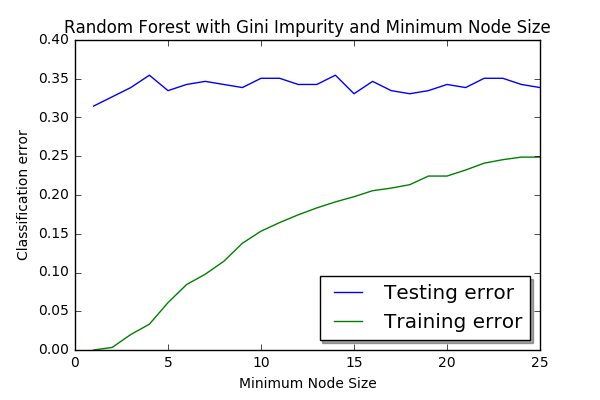
\includegraphics[width=5in]{2d.png}}
	\vspace{-10mm}
	\caption{Decision tree with varying minimum leaf node size.}
\end{figure}

\subsection{Problem E}

\begin{figure}[H]
	\makebox[\textwidth][c]{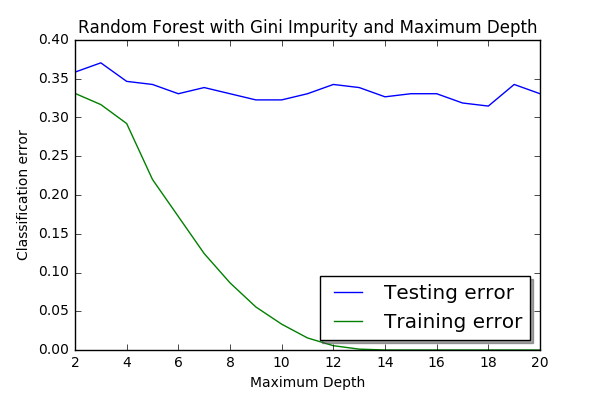
\includegraphics[width=4.2in]{2e.png}}
	\vspace{-10mm}
	\caption{Decision tree with varying maximum tree depth.}
\end{figure}

\subsection{Problem F}
Training error is minimized when the minimum node size is 1 and the maximum tree depth is 18.  Early stopping seems to have little effect on the performance of the random tree. The testing error is fairly constant for both types of early stopping.

\subsection{Problem G}
The curves for decision trees and random forests have pretty similar general shapes. The decision trees seem to have higher training error as the early stopping constraint is relaxed, but the effect is fairly small. The errors for the random forests are also generally lower than for decision trees. For reasons unknown....

\section{Problem 3}

\subsection{Problem A}
We will show that exponential loss bounds 0/1 loss.

$$E = \frac{1}{N}\sum_{i=1}^{N}exp(-y_i f(x_i))$$
$$ = \frac{1}{N}\sum_{i=1}^{N}exp\Big\{-y\{\sum_{t=1}^{n}a_th_t(x)\}\Big\}$$
$$ = \frac{1}{N}\sum_{i=1}^{N}\prod_{t=1}^n exp\{-y\alpha_th_t(x)\}$$

When $f_(x)$ is negative, the product $-y_i f(x_i)$ is positive, so the exponential term $exp(-y_if(x_i)$ is positive and greater than one. The product of positive numbers greater than one is also positive and greater than one, which bounds 0/1 loss for when $f(x) < 0$. When $f(x)$ is exactly 0, then the exponential term is 1 and the product across $n$ is 1. This is equivalent to zero one loss when $f(x) = 0$. Finally, when $f(x) < 1$ the each exponential term must still be positive, so the product is also positive and thus greater than 0.


\subsection{Problem B}

$$D_{t+1}(i) = \frac{D_t(i)exp\{-\alpha_ty_ih_t(x_i)\}}{Z_t}$$
$$D_{t+1}(i) = \frac{D_{t-1}(i)exp\{-\alpha_{t-1}y_ih_{t-1}(x_i)\}}{Z_{t-1}}\frac{exp\{-\alpha_ty_ih_t(x_i)\}}{Z_t}$$
$$D_{t+1}(i) = \frac{D_{t-2}(i)exp\{-\alpha_{t-2}y_ih_{t-2}(x_i)\}}{Z_{t-2}}\frac{exp\{-\alpha_{t-1}y_ih_{t-1}(x_i)\}}{Z_{t-1}}\frac{exp\{-\alpha_ty_ih_t(x_i)\}}{Z_t}....$$
$$D_{t+1}(i) = D_1(i)\prod_{t=1}^{T}\frac{exp\{-\alpha_ty_ih_t(x_i)\}}{Z_t}$$
$$D_{t+1}(i) = \frac{1}{N}\prod_{t=1}^{T}\frac{exp\{-\alpha_ty_ih_t(x_i)\}}{Z_t}$$





\subsection{Problem C}
$$E = \frac{1}{N}\sum_{i=1}^{N}exp(-y_i f(x_i))$$
$$E = \sum_{i=1}^{N}\frac{1}{N}exp(-y_t f(x_i))$$

Substitute $f(x) = \sum_i^T\alpha_th_t(x)$

$$E = \sum_{i=1}^{N}\frac{1}{N}exp(-y_i  \sum_t^T\alpha_th_t(x_i)))$$
$$E = \sum_{i=1}^{N}\frac{1}{N}exp(-  \sum_t^Ty_i\alpha_th_t(x_i)))$$

\subsection{Problem D}
$$E = \sum_{i=1}^{N}\frac{1}{T}exp(-  \sum_t^Ty_i\alpha_th_t(x_i)))$$
$$ = \frac{1}{N}\sum_{i=1}^{T}\prod_{t=1}^n exp\{-y\alpha_th_t(x_i)\}$$
$$ = \sum_{i=1}^{T}D_t\prod_{t=1}^{T}Z_t$$
$$ E = \prod_{t=1}^{T}Z_t$$

\subsection{Problem E}
$$Z_t = \sum_{i=1}^ND_t(i)exp(-\alpha_ty_ih_t(x_i))$$
We split this into where the points are correctly and incorrectly classified:
$$Z_t = (1-\epsilon_t) \sum_{i=1}^ND_t(i)exp(-\alpha_ty_ih_t(x_i)) + \epsilon_t\sum_{i=1}^ND_t(i)exp(-\alpha_ty_ih_t(x_i))$$
$$Z_t = (1-\epsilon_t) exp(-\alpha_t) + \epsilon_t exp(\alpha_t)$$

\subsection{Problem F}
We take the derivative of $Z_t$ with respect to $\alpha_t$, set the result to zero, and solve for $\alpha_t$.

$$\frac{\partial Z_t}{\partial\alpha_t} = 0 = - (1-\epsilon_t)exp(-\alpha_t) + \epsilon_t exp(\alpha_t)$$
$$\frac{1-\epsilon_t}{\epsilon_t} exp(-\alpha_t) = exp(\alpha_t)$$
$$\frac{1-\epsilon_t}{\epsilon_t} = exp(2\alpha_t)$$
$$\alpha_t = \frac{1}{2}ln(\frac{1-\epsilon_t}{\epsilon_t})$$

\newpage
\subsection{Problem G}

%gradient boosting
\underline{Gradient Boosting}
\begin{figure}[H]
	\makebox[\textwidth][c]{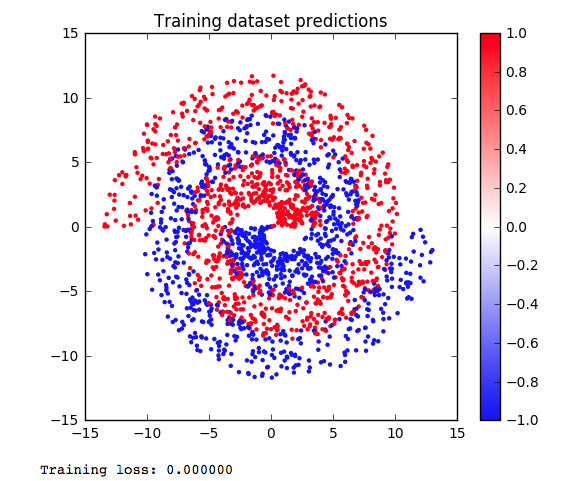
\includegraphics[width=4in]{gb_train.png}}
	\vspace{-10mm}
	\caption{Training dataset for gradient boosting}
\end{figure}

\begin{figure}[H]
	\makebox[\textwidth][c]{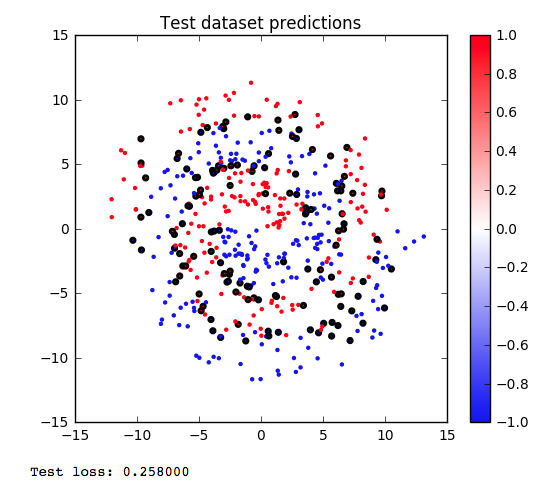
\includegraphics[width=4.2in]{gb_test.png}}
	\vspace{-10mm}
	\caption{Test dataset for gradient boosting}
\end{figure}



%Adaptive Boosting
\underline{Adaboost}
\begin{figure}[H]
	\makebox[\textwidth][c]{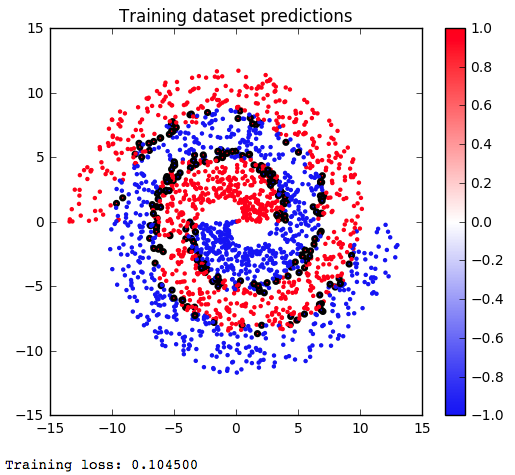
\includegraphics[width=4in]{ab_train.png}}
	\vspace{-10mm}
	\caption{Training dataset for adaptive boosting.}
\end{figure}

\begin{figure}[H]
	\makebox[\textwidth][c]{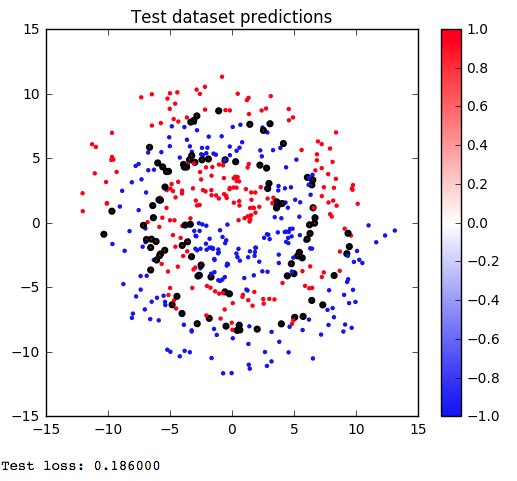
\includegraphics[width=4.2in]{ab_test.png}}
	\vspace{-10mm}
	\caption{Testing dataset for adaptive boosting}
\end{figure}



\subsection{Problem H}

\begin{figure}[H]
	\makebox[\textwidth][c]{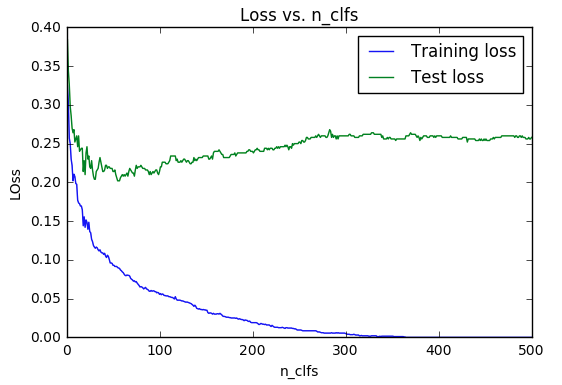
\includegraphics[width=4.8in]{gb_clf.png}}
	\vspace{-10mm}
	\caption{Learning curve for gradient boosting}
\end{figure}

\begin{figure}[H]
	\makebox[\textwidth][c]{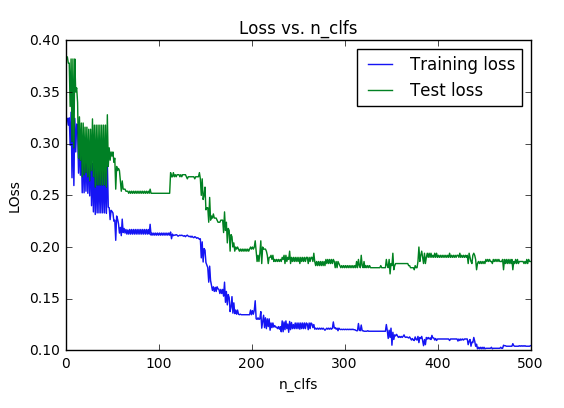
\includegraphics[width=4.8in]{adaboost_clf.png}}
	\vspace{-10mm}
	\caption{Learning curve for adaptive boosting.}
\end{figure}

The training loss for gradient boosting starts at about 0.35 and falls steadily towards zero as the number of classifiers increases. The test loss for gradient boosting begins at about the same level, falls to a minimum of about 0.2 when there are about 40 classifiers, and then increases as the number of classifiers increases. As the number of classifiers increases, overfitting occurs. The curves are fairly smooth.

The training loss for adaboost starts at about 0.32 and falls to 0.21 as the number of classifiers rises to about 50. The training loss levels off and then falls again when the number of classifiers reaches 150. After that, the training loss falls quickly to 0.12, and then falls more slowly towards 0.1. The test loss behaves similarly. The test loss begins at about 0.37, falls to 0.25 at 50 classifiers, stabilizes, then falls after 150 classifiers. Afterwards the test loss stabilizes at about 0.2. The adaboost curve is much more jagged and has sharper variations than the gradient boosting curve.


\subsection{Problem I}
The final training error of gradient boosting is about 0 and the final testing error is 0.26. The final training error of Adaboost is about 0.1 and the testing error is 0.18. The adaptive boosting algorithm performed better on the classification dataset.

\subsection{Problem J}

The dataset weights are the largest near the center of each spiral arm away from the boundaries while the weights are the smallest at the boundaries between red and blue.



\end{document}
